% Provenance (never printed): cycle 3 "La planete Terre" (natural phenomena
% and the risks they bring: storms, floods, droughts, earthquakes, eruptions;
% warnings and the right behaviour); see sources/book1/PROVENANCE.md.
% Book 1, grade 5, chapter 3.
\chapter{Natuurgevaren}\label{ch:g5:natural-hazards}

Het is vrijdagavond. Op de radio stopt de muziek en een rustige stem leest
een waarschuwing voor: vannacht bereikt een zware \omterm{def:g5:natural-hazards:storm}{storm} de \omterm{def:g1:landscapes-around-us:water}{kust}, met heel
harde wind en veel \omterm{def:g4:clouds-rain-snow:precipitation}{regen}. Mensen wordt gevraagd vanaf negen uur binnen te
blijven en alles wat de wind kan meenemen vast te zetten of naar binnen te
halen.

Lena's familie gaat aan de slag. Haar vader zet de tuinstoelen en de tafel
in het schuurtje. Haar moeder controleert of de zaklampen werken en legt
reservebatterijen op de keukentafel. Lena vult twee grote flessen met
water. Om negen uur is iedereen binnen, en de wind giert al.

\begin{omfigure}
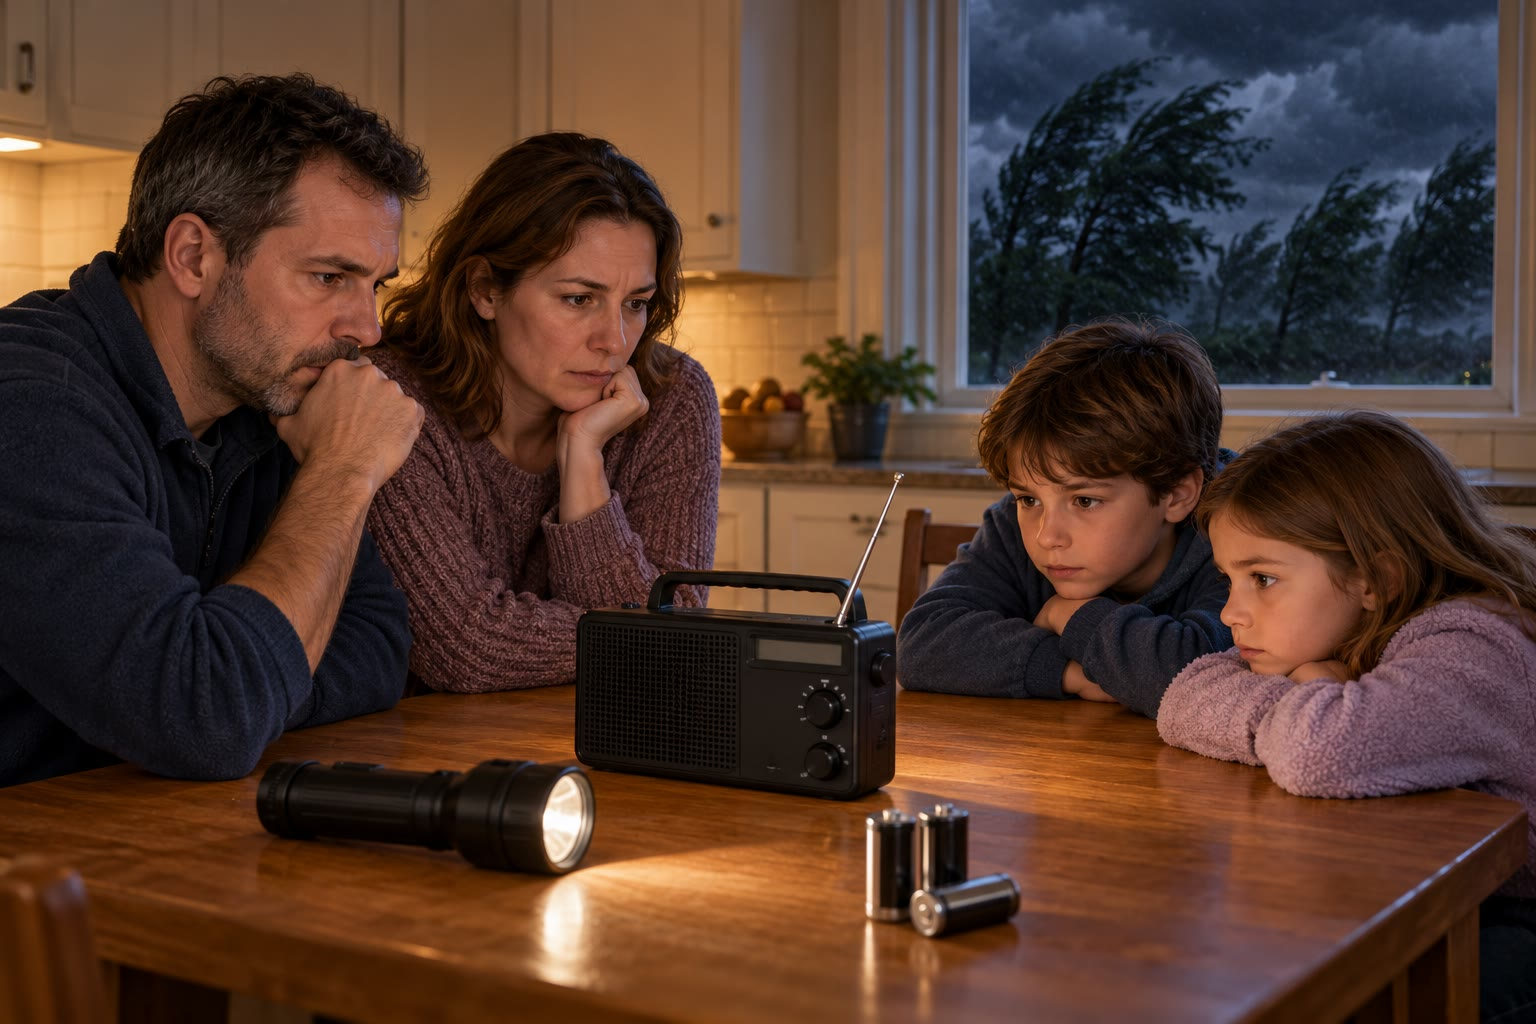
\includegraphics[width=0.5\linewidth]{images/book1/ai/g5-radio-warning.jpg}

{\small Een gezin luistert naar een stormwaarschuwing op de radio, met
zaklampen en reservebatterijen bij de hand.}
\end{omfigure}

\begin{recall}
Een \omterm{def:g4:volcanoes-earthquakes-first-look:volcano}{vulkaan} kan uitbarsten en \omterm{def:g4:volcanoes-earthquakes-first-look:eruption}{lava}, as en gas uitstoten; een \omterm{def:g4:volcanoes-earthquakes-first-look:earthquake}{aardbeving} is
een plotseling schudden van de grond; bij een \omterm{def:g4:volcanoes-earthquakes-first-look:earthquake}{aardbeving} moeten we bukken,
dekken en vasthouden (\cref{ch:g4:volcanoes-earthquakes-first-look}). Een
\omterm{def:g1:landscapes-around-us:water}{rivier} die meer water krijgt dan haar bedding kan bevatten, overstroomt
haar \omterm{def:g5:water-shapes-the-land:flood}{overstromingsvlakte} (\cref{ch:g5:water-shapes-the-land}). Elke plaats
heeft haar eigen \omterm{def:g5:weather-and-climate:climate}{klimaat}, en de warme, gematigde en koude zones lopen rond
de \omterm{def:g3:continents-and-oceans:globe}{globe} (\cref{ch:g5:weather-and-climate}).
\end{recall}

\section{Wat een natuurgevaar is}

De natuur is niet altijd rustig. De wind kan zo hard waaien dat er bomen
breken, \omterm{def:g1:landscapes-around-us:water}{rivieren} kunnen buiten hun oevers treden, de grond kan schudden.
Die gebeurtenissen horen bij de manier waarop de Aarde werkt: ze gebeurden
al lang voordat er mensen waren, en ze zullen blijven gebeuren.

\begin{definition}[Natuurgevaar]\label{def:g5:natural-hazards:hazard}
Een \emph{natuurgevaar}\index{natuurgevaar} is een natuurlijke gebeurtenis
die mensen kan treffen of kan beschadigen wat ze gebouwd hebben: een \omterm{def:g5:natural-hazards:storm}{storm},
een \omterm{def:g5:water-shapes-the-land:flood}{overstroming}, een \omterm{def:g5:natural-hazards:drought}{droogte}, een \omterm{def:g4:volcanoes-earthquakes-first-look:earthquake}{aardbeving}, een vulkaanuitbarsting, een
\omterm{def:g5:natural-hazards:landslide}{aardverschuiving}{\ldots}
\end{definition}

We kunnen \omterm{def:g5:natural-hazards:hazard}{natuurgevaren} indelen naar waar ze vandaan komen: uit de lucht,
uit het water of uit de grond.

\begin{omfigure}
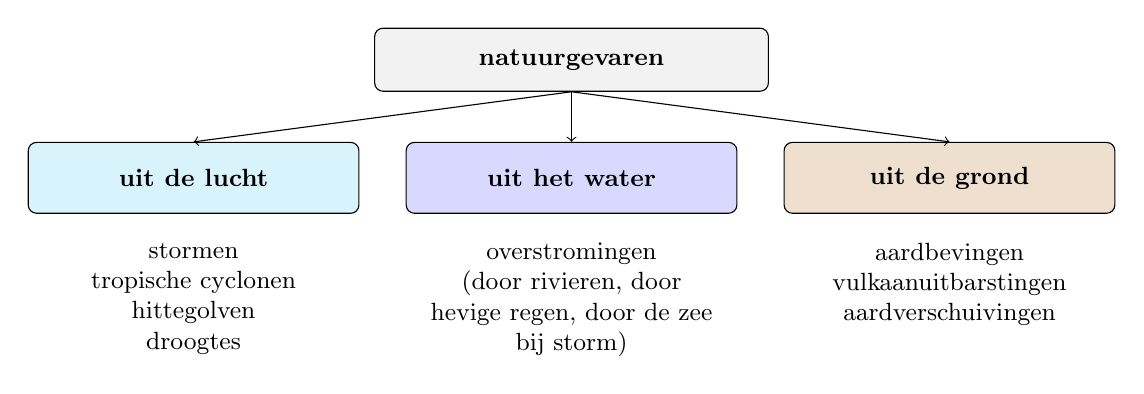
\begin{tikzpicture}[font=\small, box/.style={draw, rounded corners=3pt,
    minimum width=4.2cm, minimum height=0.9cm, align=center}]
  \node[box, fill=cyan!15, font=\small\bfseries] (A) at (0,0) {uit de lucht};
  \node[box, fill=blue!15, font=\small\bfseries] (W) at (4.8,0) {uit het water};
  \node[box, fill=brown!25, font=\small\bfseries] (G) at (9.6,0) {uit de grond};
  \node[align=center, anchor=north] at (0,-0.7) {stormen\\tropische cyclonen\\hittegolven\\droogtes};
  \node[align=center, anchor=north] at (4.8,-0.7) {overstromingen\\(door rivieren, door\\hevige regen, door de zee\\bij storm)};
  \node[align=center, anchor=north] at (9.6,-0.7) {aardbevingen\\vulkaanuitbarstingen\\aardverschuivingen};
  \node[draw, rounded corners=3pt, fill=gray!10, font=\small\bfseries,
    minimum width=5cm, minimum height=0.8cm] (N) at (4.8,1.5) {natuurgevaren};
  \draw[->] (N.south) -- (A.north);
  \draw[->] (N.south) -- (W.north);
  \draw[->] (N.south) -- (G.north);
\end{tikzpicture}

{\small De \omterm{def:g5:natural-hazards:hazard}{natuurgevaren}, ingedeeld naar waar ze vandaan komen.}
\end{omfigure}

\section{Gevaren uit de lucht}

\begin{definition}[Storm]\label{def:g5:natural-hazards:storm}
Een \emph{storm}\index{storm} is een periode met heel harde wind, meestal
met veel \omterm{def:g4:clouds-rain-snow:precipitation}{regen} of \omterm{def:g4:clouds-rain-snow:precipitation}{sneeuw}, en soms met donder en bliksem.
\end{definition}

Een zware \omterm{def:g5:natural-hazards:storm}{storm} breekt takken, blaast bomen om, rukt dakpannen van de daken
en kan tuinstoelen door ramen gooien. Aan de \omterm{def:g1:landscapes-around-us:water}{kust} stuwt de wind de \omterm{def:g2:water-on-earth:ocean}{zee} op
tegen het land en jaagt hij enorme golven over de zeeweringen.

De krachtigste \omterm{def:g5:natural-hazards:storm}{stormen} op Aarde ontstaan boven warme tropische \omterm{def:g2:water-on-earth:ocean}{zeeën}. Het
zijn enorme, draaiende \omterm{def:g5:natural-hazards:storm}{stormen}: vanuit de ruimte zien ze eruit als een
reusachtige spiraal van \omterm{def:g4:clouds-rain-snow:cloud}{wolken}, met in het midden een rustig, helder gat,
het oog. Rond het oog waaien de hardste winden. Hetzelfde soort \omterm{def:g5:natural-hazards:storm}{storm} heeft
in verschillende \omterm{def:g2:water-on-earth:ocean}{oceanen} verschillende namen: in de noordelijke
Atlantische \omterm{def:g2:water-on-earth:ocean}{Oceaan} en het oosten van de Stille \omterm{def:g2:water-on-earth:ocean}{Oceaan} heet hij een
\emph{orkaan}, in het noordwesten van de Stille \omterm{def:g2:water-on-earth:ocean}{Oceaan} een \emph{tyfoon},
en in het zuiden van de Stille \omterm{def:g2:water-on-earth:ocean}{Oceaan} en in de Indische \omterm{def:g2:water-on-earth:ocean}{Oceaan} een
\emph{tropische cycloon}.
% ledger: noaa:cyclone-names

\begin{omfigure}
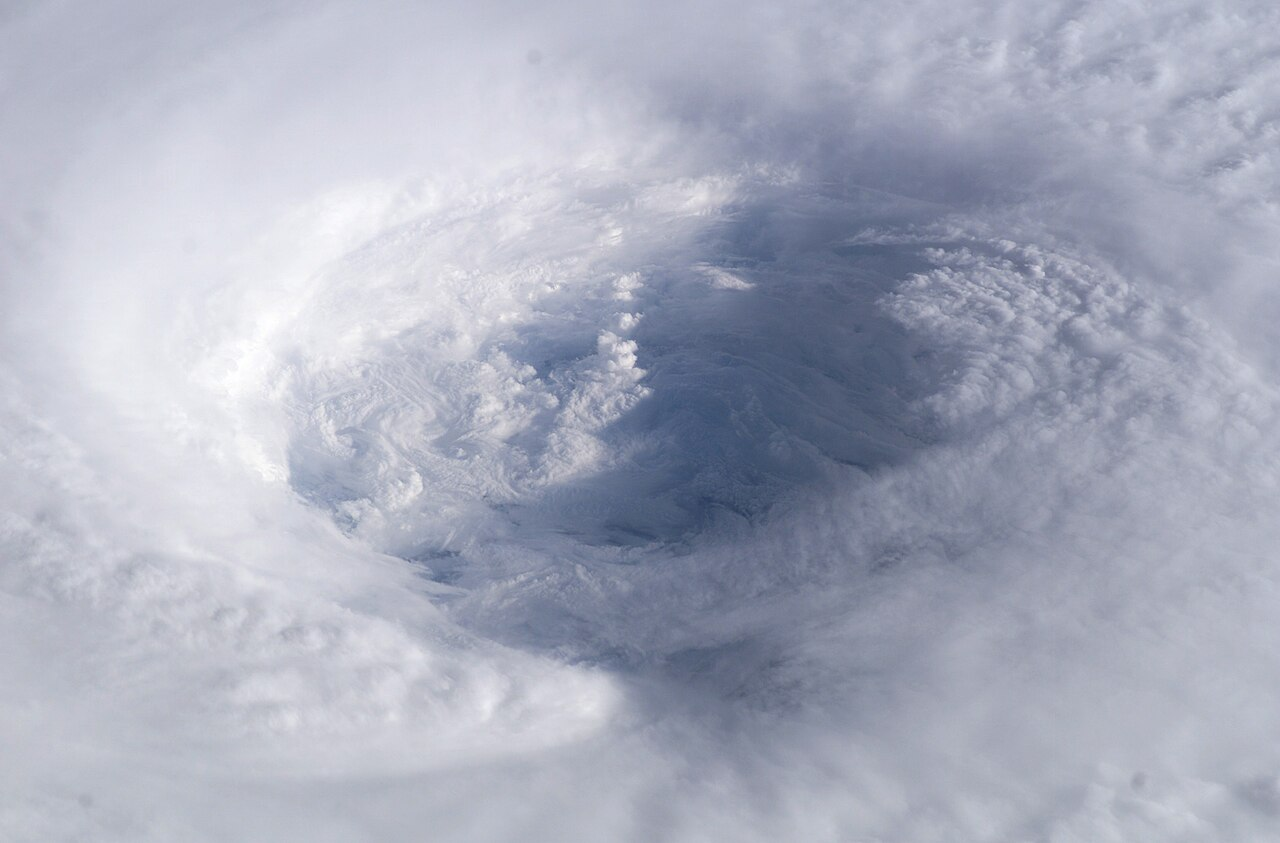
\includegraphics[width=0.5\linewidth]{images/book1/g5-hurricane-isabel-iss.jpg}

{\small Blik omlaag in het oog van orkaan Isabel, boven de Atlantische
\omterm{def:g2:water-on-earth:ocean}{Oceaan} in september 2003, vanuit het Internationaal Ruimtestation: een muur
van \omterm{def:g4:clouds-rain-snow:cloud}{wolken} rond een rustiger midden. Foto: NASA (publiek domein).}
% ledger: nasa:isabel-iss
\end{omfigure}

Sommige gevaren uit de lucht zijn traag en stil. Een \emph{hittegolf} is
een periode van een aantal dagen en nachten die veel heter zijn dan
normaal. Ze is vooral gevaarlijk voor heel oude mensen, baby's en zieken.

\begin{definition}[Droogte]\label{def:g5:natural-hazards:drought}
Een \emph{droogte}\index{droogte} is een lange periode, van maanden of zelfs
jaren, met veel minder \omterm{def:g4:clouds-rain-snow:precipitation}{regen} dan normaal voor die plaats. De bodem droogt
uit, \omterm{def:g1:landscapes-around-us:water}{rivieren} en \omterm{def:g1:landscapes-around-us:water}{meren} krimpen, gewassen verwelken en sterven af.
\end{definition}

Een \omterm{def:g5:natural-hazards:drought}{droogte} sluipt langzaam dichterbij: niemand kan zeggen op welke dag ze
begint. Maar een lange \omterm{def:g5:natural-hazards:drought}{droogte} kan boeren zonder oogst laten en steden
zonder genoeg water.

\begin{omfigure}
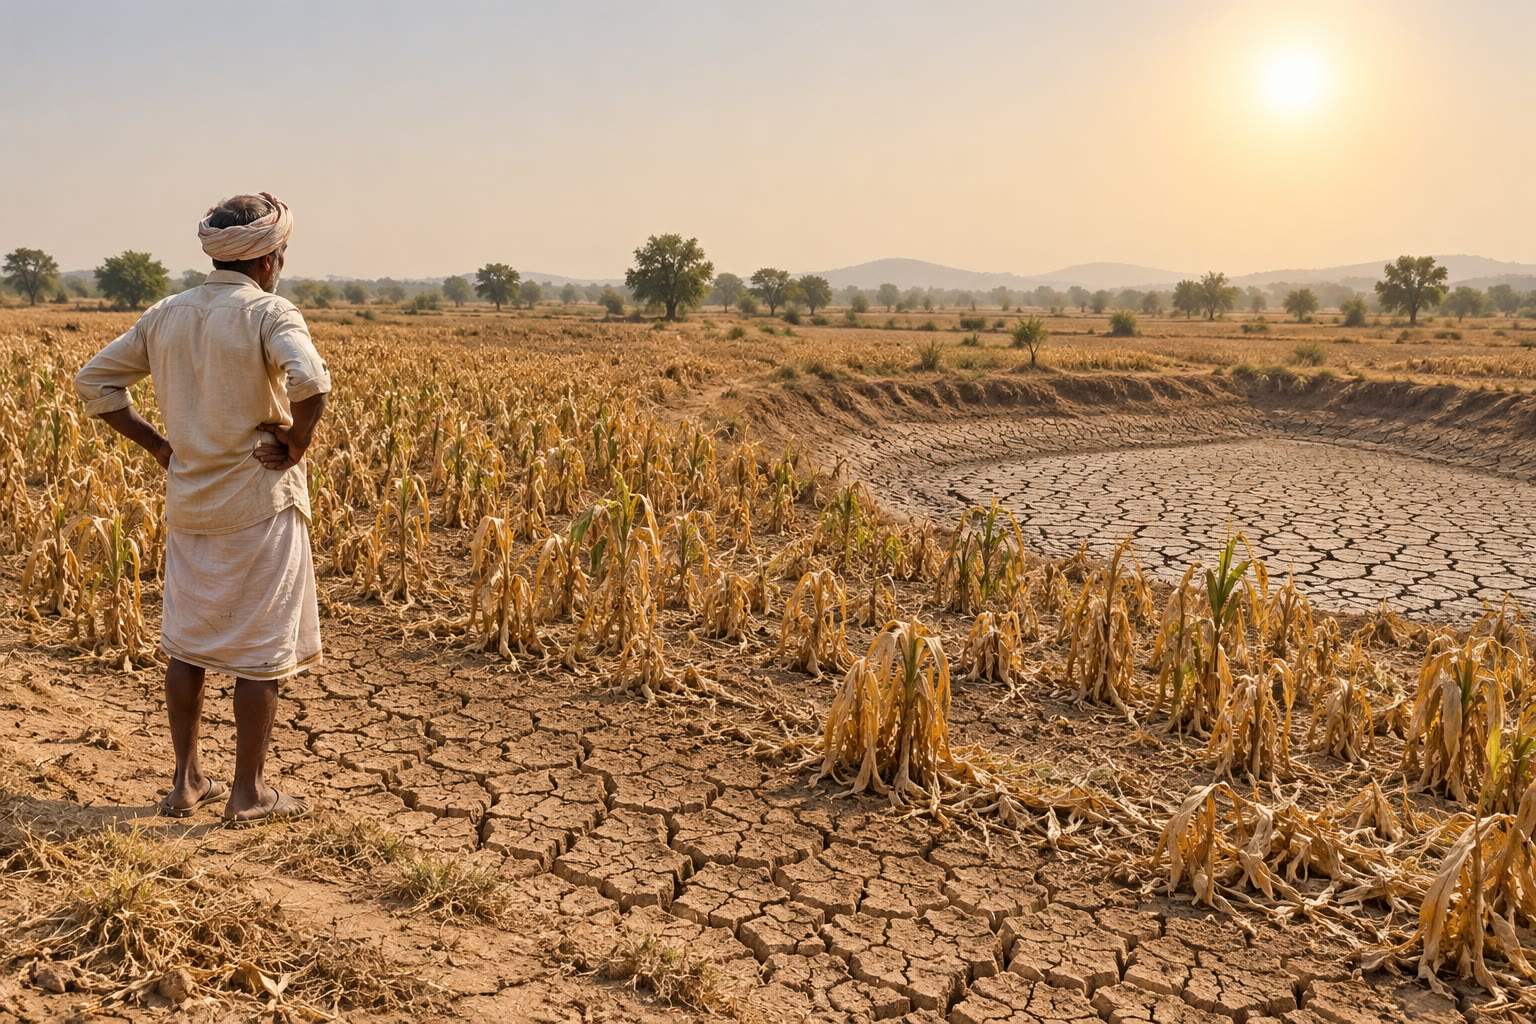
\includegraphics[width=0.42\linewidth]{images/book1/ai/g5-drought-field.jpg}

{\small Een akker tijdens een lange \omterm{def:g5:natural-hazards:drought}{droogte}: de aarde is gebarsten, de
gewassen zijn geel en de vijver is opgedroogd.}
\end{omfigure}

\section{Gevaren uit het water}

De \omterm{def:g5:water-shapes-the-land:flood}{overstromingen} van \omterm{def:g1:landscapes-around-us:water}{rivieren} ken je al (\cref{ch:g5:water-shapes-the-land}).
Na dagen \omterm{def:g4:clouds-rain-snow:precipitation}{regen}, of als de \omterm{def:g4:clouds-rain-snow:precipitation}{sneeuw} snel smelt, stijgt een \omterm{def:g1:landscapes-around-us:water}{rivier} boven haar
oevers uit en bedekt ze haar \omterm{def:g5:water-shapes-the-land:flood}{overstromingsvlakte}. Sommige \omterm{def:g5:water-shapes-the-land:flood}{overstromingen}
komen heel snel: een hevige stortbui in een steil \omterm{def:g1:landscapes-around-us:landform}{dal} kan een rustige beek
binnen een uur in een bulderende woeste stroom veranderen. Andere komen uit
de \omterm{def:g2:water-on-earth:ocean}{zee}, als een \omterm{def:g5:natural-hazards:storm}{storm} het water op een lage \omterm{def:g1:landscapes-around-us:water}{kust} opstuwt.

\section{Gevaren uit de grond}

\omterm{def:g4:volcanoes-earthquakes-first-look:earthquake}{Aardbevingen} en vulkaanuitbarstingen ken je al
(\cref{ch:g4:volcanoes-earthquakes-first-look}). Er is een derde gevaar uit
de grond, en vaak is water de aanleiding.

\begin{definition}[Aardverschuiving]\label{def:g5:natural-hazards:landslide}
Een \emph{aardverschuiving}\index{aardverschuiving} is een massa \omterm{def:g3:stones-pebbles-sand:rock}{gesteente},
aarde of modder die plotseling van een helling glijdt of valt.
\end{definition}

Een steile helling die door lange \omterm{def:g4:clouds-rain-snow:precipitation}{regens} doorweekt is, wordt zwaar en
glibberig, en kan in één keer loslaten. Ook een \omterm{def:g4:volcanoes-earthquakes-first-look:earthquake}{aardbeving} kan een helling
losschudden. Een \omterm{def:g5:natural-hazards:landslide}{aardverschuiving} kan een weg bedelven, een \omterm{def:g1:landscapes-around-us:water}{rivier}
versperren of huizen meesleuren.

\begin{omfigure}
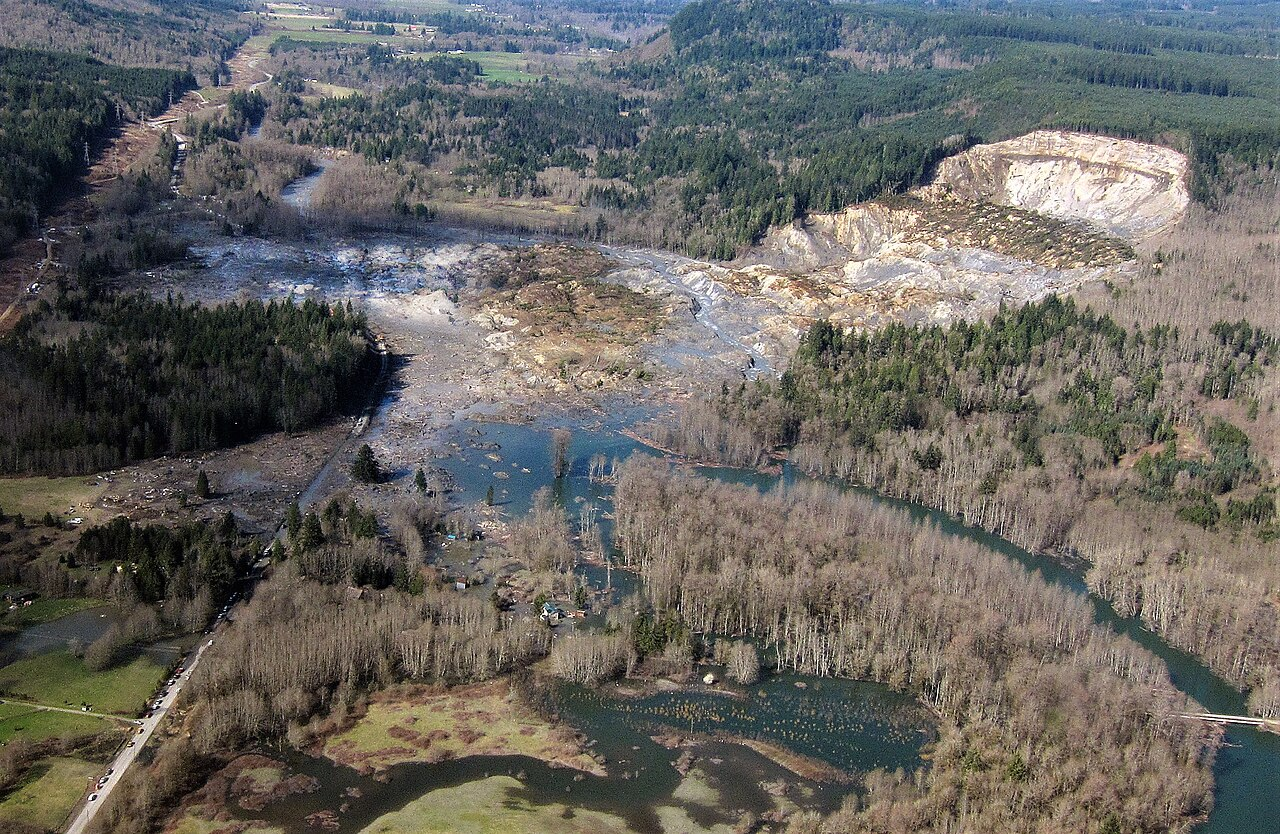
\includegraphics[width=0.6\linewidth]{images/book1/g5-landslide-washington.jpg}

{\small Een grote \omterm{def:g5:natural-hazards:landslide}{aardverschuiving} in de staat Washington, in de Verenigde
Staten, in 2014, gezien vanuit een vliegtuig. De heuvelhelling rechts is
ingestort; haar modder heeft zich over het hele \omterm{def:g1:landscapes-around-us:landform}{dal} verspreid, een weg
bedekt en de \omterm{def:g1:landscapes-around-us:water}{rivier} versperd, die stroomopwaarts het bos onder water heeft
gezet. Foto: Mark Reid, U.S. Geological Survey (publiek domein).}\label{fig:g5:natural-hazards:landslide}
% ledger: usgs:oso-aerial
\end{omfigure}

\section{Van gevaar tot ramp}

Een \omterm{def:g5:natural-hazards:storm}{storm} boven de open \omterm{def:g2:water-on-earth:ocean}{oceaan}, een \omterm{def:g4:volcanoes-earthquakes-first-look:earthquake}{aardbeving} in een lege \omterm{def:g5:weather-and-climate:desert}{woestijn}, een
\omterm{def:g5:water-shapes-the-land:flood}{overstroming} in een \omterm{def:g1:landscapes-around-us:landform}{dal} waar niemand woont: dat zijn \omterm{def:g5:natural-hazards:hazard}{natuurgevaren}, maar
ze treffen niemand. Dezelfde gebeurtenissen worden gevaarlijk als ze
toeslaan waar mensen wonen.

\begin{definition}[Natuurramp]\label{def:g5:natural-hazards:disaster}
Er is een \emph{natuurramp}\index{natuurramp} als een \omterm{def:g5:natural-hazards:hazard}{natuurgevaar} toeslaat
op een plaats waar mensen wonen en grote schade aanricht: mensen raken
gewond of komen om, huizen worden verwoest, wegen, water en elektriciteit
vallen weg.
\end{definition}

\begin{omfigure}
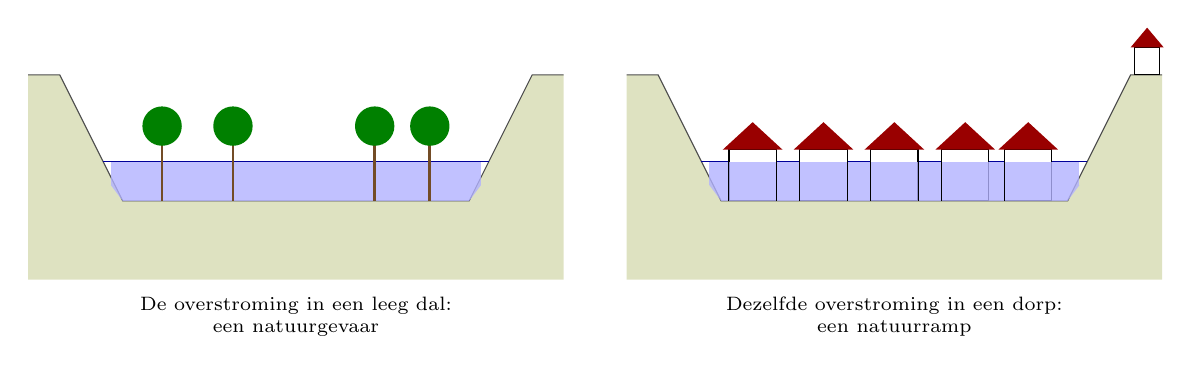
\begin{tikzpicture}[x=1cm, y=1cm, font=\scriptsize]
  \foreach \dx/\title in {0/{De overstroming in een leeg dal:\\een natuurgevaar},
                          7.6/{Dezelfde overstroming in een dorp:\\een natuurramp}} {
    \begin{scope}[xshift=\dx cm]
      % valley sides
      \fill[green!25!brown!30] (0,0) -- (0,2.6) -- (0.4,2.6) -- (1.2,1.0) -- (5.6,1.0)
        -- (6.4,2.6) -- (6.8,2.6) -- (6.8,0) -- cycle;
      \draw[gray!60!black] (0,2.6) -- (0.4,2.6) -- (1.2,1.0) -- (5.6,1.0) -- (6.4,2.6) -- (6.8,2.6);
      % flood water over the whole valley floor
      \fill[blue!30, opacity=0.8] (1.05,1.2) -- (5.75,1.2) -- (5.6,1.0) -- (1.2,1.0) -- cycle;
      \fill[blue!30, opacity=0.8] (1.05,1.2) rectangle (5.75,1.5);
      \draw[blue!60!black] (0.95,1.5) -- (5.85,1.5);
      \node[align=center, anchor=north] at (3.4,-0.1) {\title};
    \end{scope}
  }
  % trees in the empty valley
  \foreach \x in {1.7,2.6,4.4,5.1} {
    \draw[brown!60!black, line width=1pt] (\x,1.0) -- (\x,1.75);
    \fill[green!50!black] (\x,1.95) circle (0.25);
  }
  % houses in the village valley
  \begin{scope}[xshift=7.6cm]
    \foreach \x in {1.6,2.5,3.4,4.3,5.1} {
      \fill[white, draw=black] (\x-0.3,1.0) rectangle (\x+0.3,1.65);
      \fill[red!60!black] (\x-0.38,1.65) -- (\x,2.0) -- (\x+0.38,1.65) -- cycle;
      \fill[blue!30, opacity=0.8] (\x-0.3,1.0) rectangle (\x+0.3,1.5);
    }
    % one house on the high ground, dry
    \fill[white, draw=black] (6.45,2.6) rectangle (6.77,2.95);
    \fill[red!60!black] (6.40,2.95) -- (6.61,3.2) -- (6.82,2.95) -- cycle;
  \end{scope}
\end{tikzpicture}

{\small Twee keer dezelfde \omterm{def:g5:water-shapes-the-land:flood}{overstroming}. In het lege \omterm{def:g1:landscapes-around-us:landform}{dal} treft ze niemand;
waar een dorp op de \omterm{def:g5:water-shapes-the-land:flood}{overstromingsvlakte} is gebouwd, lopen de huizen vol. Het
huis op de hoge grond blijft droog.}
\end{omfigure}

We kunnen een \omterm{def:g5:natural-hazards:storm}{storm} of een \omterm{def:g4:volcanoes-earthquakes-first-look:earthquake}{aardbeving} niet tegenhouden. Maar we kunnen veel
doen om te voorkomen dat een gevaar een ramp wordt: bouwen buiten
\omterm{def:g5:water-shapes-the-land:flood}{overstromingsvlakten} en niet aan de voet van onstabiele hellingen,
gebouwen stevig maken, het \omterm{def:g1:watching-the-weather:weather}{weer} en de grond in de gaten houden, mensen op
tijd waarschuwen, en iedereen leren wat te doen.

\subsection*{Waarschuwingen}

Weerdiensten houden de lucht dag en nacht in de gaten. Als er een \omterm{def:g5:natural-hazards:storm}{storm},
een hittegolf of een \omterm{def:g5:water-shapes-the-land:flood}{overstroming} aankomt, sturen ze waarschuwingen uit via
radio, televisie, telefoon en internet. Veel landen gebruiken kleuren, van
de rustigste tot de ernstigste.

\begin{omfigure}
\begin{tikzpicture}[font=\small, wstep/.style={draw=black!60, minimum width=2.6cm,
    minimum height=0.8cm, font=\small\bfseries, rounded corners=2pt}]
  \node[wstep, fill=green!45] (g) at (0,0) {groen};
  \node[wstep, fill=yellow!60] (y) at (0.6,0.95) {geel};
  \node[wstep, fill=orange!70] (o) at (1.2,1.9) {oranje};
  \node[wstep, fill=red!65, text=white] (r) at (1.8,2.85) {rood};
  \node[anchor=west] at ($(g.east)+(0.3,0)$) {geen bijzonder gevaar};
  \node[anchor=west] at ($(y.east)+(0.3,0)$) {wees voorzichtig, blijf op de hoogte};
  \node[anchor=west] at ($(o.east)+(0.3,0)$) {wees voorbereid: gevaar is waarschijnlijk};
  \node[anchor=west] at ($(r.east)+(0.3,0)$) {groot gevaar: kom nu in actie, volg de instructies};
\end{tikzpicture}

{\small Een ladder van waarschuwingskleuren. De precieze betekenis verschilt
van land tot land: luister altijd naar de instructies die bij de
waarschuwing horen.}
\end{omfigure}

\begin{safety}
\textbf{Bij \omterm{def:g5:natural-hazards:storm}{storm}.} Blijf binnen, uit de buurt van ramen. Ga niet naar
buiten om te kijken, en blijf weg bij bomen, die kunnen omvallen, en bij
afgebroken elektriciteitsdraden.

\textbf{Bij een \omterm{def:g5:water-shapes-the-land:flood}{overstroming}.} Ga naar hoger gelegen grond of naar een
hogere verdieping. Loop, fiets of rijd nooit door overstromingswater: een
beetje snel stromend water is genoeg om je omver te duwen of een auto mee
te sleuren.

\textbf{Bij een hittegolf.} Drink vaak water, blijf tijdens de heetste uren
in de schaduw of in een koele kamer, en ga na of het goed gaat met oudere
buren.

\textbf{Bij een \omterm{def:g4:volcanoes-earthquakes-first-look:earthquake}{aardbeving}.} Bukken, dekken, vasthouden
(\cref{ch:g4:volcanoes-earthquakes-first-look}).

\textbf{Altijd.} Luister naar de waarschuwingen en doe meteen wat de mensen
die de leiding hebben zeggen.
\end{safety}

\section{Oefeningen}

\begin{exercise}[$\star$]\label{exo:g5:natural-hazards:1}
Alleen een \omterm{def:g5:natural-hazards:hazard}{natuurgevaar}, of een \omterm{def:g5:natural-hazards:disaster}{natuurramp}?
\begin{enumerate}
  \item[(a)] Een \omterm{def:g4:volcanoes-earthquakes-first-look:earthquake}{aardbeving} doet een lege \omterm{def:g5:weather-and-climate:desert}{woestijn} schudden.
  \item[(b)] Een \omterm{def:g5:natural-hazards:storm}{storm} rukt in een stad de daken van veel huizen.
  \item[(c)] Een \omterm{def:g5:natural-hazards:landslide}{aardverschuiving} valt in een bergdal waar niemand woont.
  \item[(d)] Een \omterm{def:g1:landscapes-around-us:water}{rivier} overstroomt een dorp en de huizen lopen vol water.
\end{enumerate}
\end{exercise}

\begin{exercise}[$\star$]\label{exo:g5:natural-hazards:2}
Deel deze gevaren in drie families in (uit de lucht, uit het water, uit de
grond): een \omterm{def:g5:natural-hazards:landslide}{aardverschuiving}; een hittegolf; een \omterm{def:g5:water-shapes-the-land:flood}{overstroming}; een
vulkaanuitbarsting; een \omterm{def:g5:natural-hazards:storm}{storm}; een \omterm{def:g5:natural-hazards:drought}{droogte}; een \omterm{def:g4:volcanoes-earthquakes-first-look:earthquake}{aardbeving}.
\end{exercise}

\begin{exercise}[$\star$]\label{exo:g5:natural-hazards:3}
Wat is een \omterm{def:g5:natural-hazards:drought}{droogte}? Noem twee manieren waarop een lange \omterm{def:g5:natural-hazards:drought}{droogte} mensen treft.
\end{exercise}

\begin{exercise}[$\star$]\label{exo:g5:natural-hazards:4}
De radio kondigt voor vannacht code rood voor \omterm{def:g5:natural-hazards:storm}{storm} aan. Noem drie dingen
die je gezin moet doen.
\end{exercise}

\begin{exercise}[$\star$]\label{exo:g5:natural-hazards:5}
Boven een warme tropische \omterm{def:g2:water-on-earth:ocean}{zee} ontstaat een grote draaiende \omterm{def:g5:natural-hazards:storm}{storm} met een
oog. Hoe heet hij als hij toeslaat op (a) de \omterm{def:g1:landscapes-around-us:water}{kust} van Florida, in de
noordelijke Atlantische \omterm{def:g2:water-on-earth:ocean}{Oceaan}; (b) Japan, in het noordwesten van de Stille
\omterm{def:g2:water-on-earth:ocean}{Oceaan}; (c) de \omterm{def:g1:landscapes-around-us:water}{kust} van India, aan de Indische \omterm{def:g2:water-on-earth:ocean}{Oceaan}?
\end{exercise}

\begin{exercise}[$\star$]\label{exo:g5:natural-hazards:6}
Zet de vier waarschuwingskleuren op volgorde, van de rustigste tot de
ernstigste. Wat moet je doen bij het ernstigste niveau?
\end{exercise}

\begin{exercise}[$\star\star$]\label{exo:g5:natural-hazards:7}
Kijk naar de foto van de \omterm{def:g5:natural-hazards:landslide}{aardverschuiving} op
bladzijde~\pageref{fig:g5:natural-hazards:landslide}. Beschrijf wat de
\omterm{def:g5:natural-hazards:landslide}{aardverschuiving} met het \omterm{def:g1:landscapes-around-us:landform}{dal} heeft gedaan: met de heuvelhelling, met de weg
en met de \omterm{def:g1:landscapes-around-us:water}{rivier}. Waarom staat het land stroomopwaarts nu onder water?
\end{exercise}

\begin{exercise}[$\star\star$]\label{exo:g5:natural-hazards:8}
Tom zegt: ``\omterm{def:g5:water-shapes-the-land:flood}{Overstromingen} zijn natuurlijk, dus je kunt er niets aan
doen.'' Lena zegt: ``We kunnen een \omterm{def:g1:landscapes-around-us:water}{rivier} niet tegenhouden als ze
overstroomt, maar we kunnen voorkomen dat een \omterm{def:g5:water-shapes-the-land:flood}{overstroming} een ramp wordt.''
Wie heeft gelijk? Leg uit met twee voorbeelden.
\end{exercise}

\begin{exercise}[$\star\star$]\label{exo:g5:natural-hazards:9}
In een denkbeeldige landbouwstreek valt er gewoonlijk ongeveer
60 millimeter \omterm{def:g4:clouds-rain-snow:precipitation}{regen} per maand. Tijdens een \omterm{def:g5:natural-hazards:drought}{droogte} viel er vier maanden
lang elke maand maar een kwart van de gewone \omterm{def:g4:clouds-rain-snow:precipitation}{regen}.
\begin{enumerate}
  \item[(a)] Hoeveel \omterm{def:g4:clouds-rain-snow:precipitation}{regen} valt er gewoonlijk in vier maanden?
  \item[(b)] Hoeveel viel er tijdens de \omterm{def:g5:natural-hazards:drought}{droogte}, in de vier maanden?
  \item[(c)] Hoeveel \omterm{def:g4:clouds-rain-snow:precipitation}{regen} ontbrak er?
\end{enumerate}
\end{exercise}

\begin{exercise}[$\star\star$]\label{exo:g5:natural-hazards:10}
Een denkbeeldige stad heeft 1\,200 woningen. Een kwart daarvan staat op de
\omterm{def:g5:water-shapes-the-land:flood}{overstromingsvlakte} van haar \omterm{def:g1:landscapes-around-us:water}{rivier}.
\begin{enumerate}
  \item[(a)] Hoeveel woningen staan er op de \omterm{def:g5:water-shapes-the-land:flood}{overstromingsvlakte}?
  \item[(b)] De stad helpt de eigenaars van een derde van die woningen om
        naar hoger gelegen grond te verhuizen. Hoeveel woningen staan er
        dan nog op de \omterm{def:g5:water-shapes-the-land:flood}{overstromingsvlakte}?
\end{enumerate}
\end{exercise}

\begin{exercise}[$\star\star\star$]\label{exo:g5:natural-hazards:11}
Twee dorpen, ver van elkaar, worden in dezelfde nacht getroffen door even
zware \omterm{def:g5:natural-hazards:storm}{stormen}. In het eerste raakt niemand gewond en is de schade klein. In
het tweede worden veel huizen verwoest. Geef minstens drie verschillende
redenen die het verschil kunnen verklaren.
\end{exercise}
